\thispagestyle{hoccungpinone}
\pagestyle{hoccungpi}
\everymath{\color{hoccungpi}}
\graphicspath{{../hoccungpi/pic/}}
\blfootnote{$^{1}$\color[named]{hoccungpi}THPT chuyên Nguyễn Quang Diêu -- Đồng Tháp.}
\begingroup
\AddToShipoutPicture*{\put(0,616){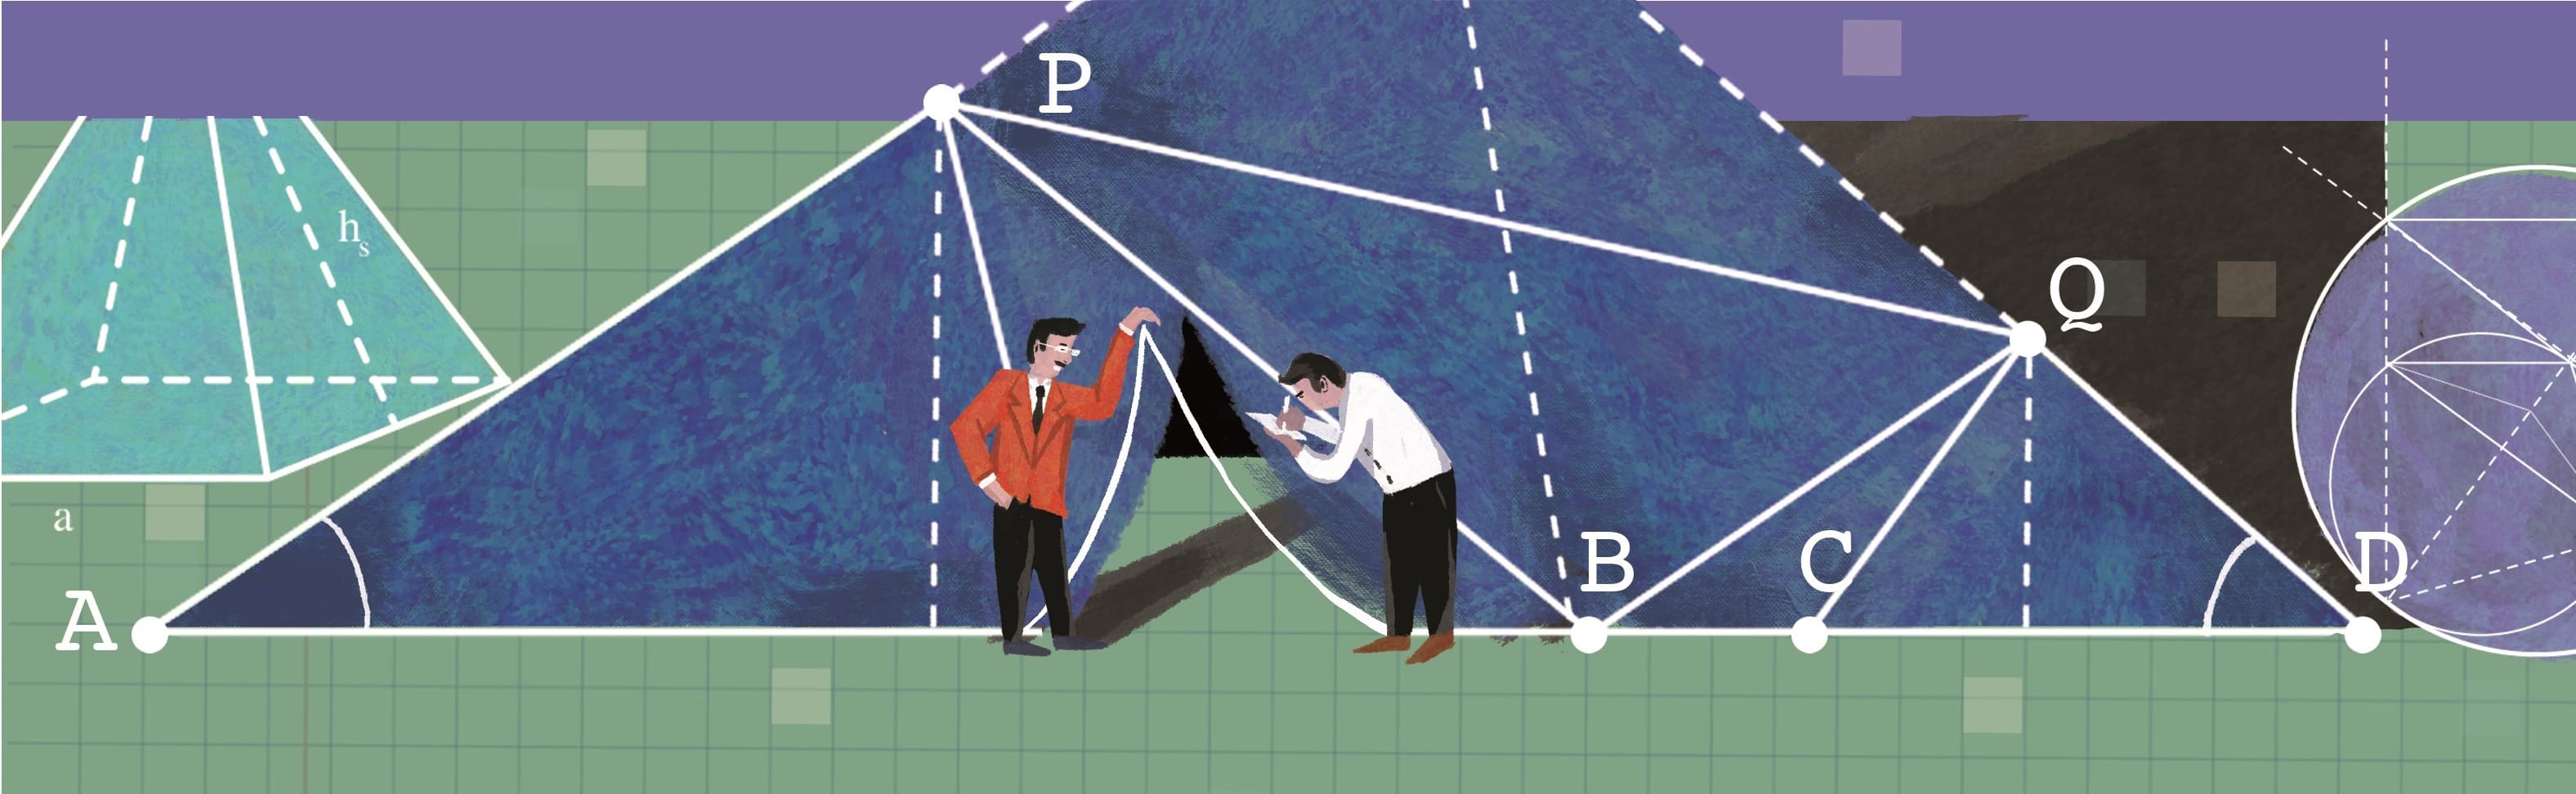
\includegraphics[width=19.3cm]{../bannerhoccungpi}}}
\AddToShipoutPicture*{\put(98,522){
\includegraphics[scale=1]{../tieude1.pdf}}}
\centering
\endgroup
\vspace*{188pt}

\begin{multicols}{2}
		\textbf{\color{hoccungpi}Giới thiệu}
		\vskip 0.1cm
		Trong tạp chí Pi tháng $10$ năm $2021$, tác giả Trần Nam Dũng  giới thiệu đến bất đẳng thức Bernoulli, ở đó tác giả có đề cập đến việc bất đẳng thức Cauchy (hay còn gọi là bất đẳng thức trung bình cộng và trung bình nhân) tương đương với bất đẳng thức Bernoulli. Bài viết này sẽ tổng hợp nhiều hơn các bất đẳng thức tương đương như vậy cũng như một số chứng minh đặc sắc có liên quan. Bài viết kết thúc với một số bài toán xuất hiện trong các kỳ thi Olympic mà ở đó bất đẳng thức Bernoulli có vai trò then chốt trong lời giải.
		\vskip 0.1cm
		$\pmb{1.}$ \textbf{\color{hoccungpi}Một số bất đẳng thức tương đương với bất đẳng thức Bernoulli}
		\vskip 0.1cm
		Nhắc lại rằng bất đẳng thức Bernoulli cho số mũ thực được phát biểu như sau (xem [$1$, Định lý $2$]: Cho số thực $x > -1$ và số thực $\alpha$. Khi đó, 
		\vskip 0.1cm
		$(1)$ Với $0 < \alpha < 1$, ta có  $(1+x)^\alpha \le 1 + \alpha x$.
		\vskip 0.1cm
		$(2)$ Với  $\alpha > 1$ hoặc $\alpha < 0$, ta có  $(1+x)^\alpha \ge 1 + \alpha x$.
		\vskip 0.1cm
		Dấu ``$=$" xảy ra khi và chỉ khi $x = 0$.
		\vskip 0.1cm
		Chúng ta sẽ bắt đầu với  kết quả sau đây.
		\vskip 0.1cm
		\textbf{\color{hoccungpi}Định lý} $\pmb{1.}$ \textit{Các mệnh đề sau là tương đương:
		\vskip 0.1cm
		$(a)$ Với $x>-1$ và $\alpha \in (0;1)$ thì $(1+x)^{\alpha} \le 1+\alpha x.$
		\vskip 0.1cm
		$(b)$ Với mọi số thực dương $\alpha, x,y$, trong đó $\alpha \in (0;1)$, ta có
		$x^{\alpha}y^{1-\alpha} \le \alpha x +(1-\alpha)y.$
		\vskip 0.1cm
		$(c)$ Hàm số $y=\ln x$ là hàm lõm trên $(0;+\infty)$. (Ở đây, ta nói một hàm số $f$ trên khoảng $I$ là lõm nếu với mọi $x, y\in I$ và $\alpha \in (0, 1)$ thì $f(\alpha x+(1-\alpha) y) \ge \alpha f(x) + (1-\alpha)f(y)$.\footnote[2]{\color{hoccungpi}Lưu ý rằng định nghĩa này khác với một số tài liệu, trong đó hàm số như vậy được gọi là lồi!})
		\vskip 0.1cm
		$(d)$ (Bất đẳng thức Young.) Với $x,y,p,q$ là các số thực dương thỏa mãn
		$\dfrac{1}{p}+\dfrac{1}{q}=1$ thì 
		\begin{align*}
			xy \le \dfrac{x^{p}}{p}+\dfrac{y^{q}}{q}.
		\end{align*}}
		\textit{Chứng minh.}
		\setlength{\abovedisplayskip}{7.2pt}
		\setlength{\belowdisplayskip}{7.2pt}
		\vskip 0.1cm
		$\bullet$ $(a) \Rightarrow (b)$.  Thay $x+1$ bằng $x$ vào bất đẳng thức (a) ta có $x^{\alpha} \le 1+\alpha(x-1)$, hay 
		\begin{align*}
			x^{\alpha} \le (1-\alpha) + \alpha x
		\end{align*}
		với mọi $ x>0,\alpha \in (0;1)$. Nhân cả hai vế của bất đẳng thức vừa nhận được với số thực dương $y$ ta được:
		\begin{align*}
			x^{\alpha}y \le (1-\alpha)y + \alpha xy.
		\end{align*}
		(Bất đẳng thức này đúng với mọi $x>0, y>0, \alpha \in (0;1)$.) Thay $x$ bằng $\dfrac{x}{y}$ vào bất đẳng thức này, ta thu được:
		\begin{align*}
			x^{\alpha}y^{1-\alpha} \le (1-\alpha)y + \alpha x,
		\end{align*}
		nghĩa là bất đẳng thức $(b)$ là đúng.
		\vskip 0.1cm
		$\bullet$ $(b) \Rightarrow (c)$ Sử dụng định nghĩa của hàm lõm.
		\vskip 0.1cm
		$\bullet$ $(c) \Rightarrow (d)$. Vì $y=\ln x$ là hàm lõm nên:
		\begin{align*}
			\ln \left( {\frac{1}{p}{x^p} + \frac{1}{q}{y^q}} \right) \ge   \frac{1}{p}\ln {x^p} + \frac{1}{q}\ln {x^q},
		\end{align*}
		do đó
		\begin{align*}
			\frac{{{x^p}}}{p} + \frac{{{y^q}}}{q} \ge xy,
		\end{align*}
		hay nói cách khác, $(d)$ đúng.
		\vskip 0.1cm
		$\bullet$ $(d) \Rightarrow (a)$. Xét $\alpha \in (0;1)$. Khi đó tồn tại số thực $p>1$ sao cho $\dfrac{1}{p}=\alpha$. Đặt $1-\alpha=\dfrac{1}{q}$ (như vậy $q>1$). Thay $x, y$ tương ứng bởi $x^p, y^q$ vào bất đẳng thức Young ta nhận được
		\begin{align*}
			x^{\alpha}y^{1-\alpha} \le \alpha x + (1-\alpha)y.
		\end{align*}
		Bất đẳng thức này đúng với mọi số thực $ x,y>0,\alpha \in (0;1)$. Đặc biệt, với $y=1$ ta được:
		\begin{align*}
			x^{\alpha} \le \alpha x + (1-\alpha),
		\end{align*}
		với mọi $x,\alpha \in (0;1)$, hay nói cách khác:
		\begin{align*}
			x^{\alpha} \le 1+\alpha (x-1).
		\end{align*}
		Thay $x$ bằng $x+1$, ta thu được:
		\begin{align*}
			(x+1)^{\alpha} \le 1+\alpha x
		\end{align*}
		với mọi $x>-1,\alpha \in (0;1)$. Vậy $(a)$ đúng.
		\vskip 0.1cm
		Tóm lại
			$(a) \Leftrightarrow (b) \Leftrightarrow (c) \Leftrightarrow (d).$
		\vskip 0.1cm
		Tiếp theo, tác giả xin trình bày một mạch tương đương dài hơn giữa nhiều bất đẳng thức quen thuộc với bất đẳng thức Bernoulli.
		\vskip 0.1cm
		\textbf{\color{hoccungpi}Định lý} $\pmb{2.}$
		\textit{Các mệnh đề sau là tương đương:
		\vskip 0.1cm
		$(T_1)$: Với $x>-1,\alpha \geq 1$ thì $(1+x)^{\alpha} \geq 1+\alpha x.$
		\vskip 0.1cm
		$(T_2)$: Với $x>-1,\alpha \leq 0$ thì
		$(1+x)^{\alpha} \geq 1+\alpha x.$
		\vskip 0.1cm
		$(T_3)$: Với $x>-1,0 \le \alpha \le 1$ thì
		$(1+x)^{\alpha} \le 1+\alpha x.$
		\vskip 0.1cm
		$(T_4)$: Với mọi số nguyên dương $n$ và các số thực $a_i,q_i>0$ ($1\le i \le n$), $ \alpha \geq 1$ thỏa mãn  $\sum_{i=1}^n q_i=1$ thì
		\begin{align*}
			\sum_{i=1}^n q_i a_i^{\alpha} \leq \left(\sum_{i=1}^n q_i a_i
			\right)^{\alpha}.
		\end{align*}
		$(T_5)$: Với mọi số nguyên dương $n$ và các số thực$a_i,q_i>0$ ($1\le i \le n$), $ \alpha \geq 1$ thỏa  mãn  $\sum_{i=1}^n q_i=1$ thì
		\begin{align*}
			\sum_{i=1}^n q_i a_i^{\alpha} \geq \left(\sum_{i=1}^n q_i a_i
			\right)^{\alpha}.
		\end{align*}
		$(T_6)$: Với mọi số nguyên dương $n$ và các số thực dương $a_i,p_i$ ($1\le i \le n$), định nghĩa $M_r$ ($r>0$) như sau:
		\begin{align*}
			M_{r}\!=\!\begin{cases}
				\!\!\left(\dfrac{p_{1} a_{1}^{r}+p_{2} a_{2}^{r}+\ldots+p_{n} a_{n}^{r}}{p_{1}+p_{2}+\ldots+p_{n}}\right)^{\frac{1}{r}}\!\!\!\!, r \neq 0 \\[+1ex]
				\left(a_{1}^{p_{1}} a_{2}^{p_{2}} \cdots a_{n}^{p_{n}}\right)^{\frac{1}{p_{1}+p_{2}+\cdots+p_{n}}}, r=0
			\end{cases}
		\end{align*}
		Khi đó, với mọi $r<s$ thì
		\begin{align*}
			M_{r} \leq M_{s}.
		\end{align*}
		$(T_7)$: (Bất đẳng thức Holder.) Với mọi số nguyên dương $n$ và các số thực dương $a_i,b_i$ ($1\le i \le n$), $p,q$ thỏa mãn $\dfrac{1}{p}+\dfrac{1}{q}=1.$ Khi đó:
		\begin{align*}
			\sum_{i=1}^{n} a_{i} b_{i} \leq\left(\sum_{i=1}^{n} a_{i}^{p}\right)^{\frac{1}{p}}\left(\sum_{i=1}^{n} b_{i}^{q}\right)^{\frac{1}{q}}.
		\end{align*}
		$(T_8)$: (Bất đẳng thức Cauchy--Schwarz.) Với mọi số nguyên dương $n$ và các số thực dương $a_i,b_i$ ($1\le i \le n$) thì
		\begin{align*}
			\left(\sum_{i=1}^{n} a_{i} b_{i}\right)^{2} \leq\left(\sum_{i=1}^{n} a_{i}^{2}\right)\left(\sum_{i=1}^{n} b_{i}^{2}\right).
		\end{align*}
		$(T_{9})$: Với mọi số thực dương $a,b$,
		\begin{align*}
			\dfrac{1}{2}\ln a+\dfrac{1}{2}\ln b \le \ln \left(\dfrac{a+b}{2} \right).
		\end{align*}
		$(T_{10})$: Với mọi số nguyên dương $n$ và các số thực dương $a_i,p_i$ ($1\le i \le n$) thì
		\begin{align*}
			\dfrac{\sum_{i=1}^n p_i\ln a_i}{\sum_{i=1}^n p_i} \le \ln \left(\dfrac{ \sum_{i=1}^n p_ia_i}{\sum_{i=1}^n p_i} \right).
		\end{align*}
		$(T_{11})$: Với mọi số nguyên dương $n$ và các số thực dương $a_i,p_i$ ($1\le i \le n$) thì
		\begin{align*}
			\prod_{i=1}^{n} a_{i}^{\frac{p_{i}}{\sum_{k=1}^{n} p_{k}}} \leq \dfrac{\sum_{i=1}^{n} p_{i} a_{i}}{\sum_{k=1}^{n} p_{k}}.
		\end{align*}
		$(T_{12})$:  Với mọi số nguyên dương $m, n$ và các số thực
		dương $\alpha_{j}, \beta_{i}$ $(1\le i \le n, 1\le j \le m$) thỏa mãn $\sum_{j=1}^{n} \alpha_{j}=\sum_{i=1}^{m} \beta_{i}=1$, định nghĩa
		\begin{align*}
			&G_{i}=a_{i,1}^{\alpha_{1}} a_{i, 2}^{\alpha_{2}} \cdots a_{i,n}^{\alpha_{n}} \\
			\text{và } &A_{j}=\beta_{1} a_{1,j}+\beta_{2} a_{2,j}+\cdots+\beta_{m} a_{m,j},
		\end{align*}
		(với $i=1,2, \ldots, m$; $j=1,2, \ldots, n$ và \linebreak$a_{k,l}>0$).
		Khi đó:
		\begin{align*}
			\sum_{i=1}^{m} \beta_{i} G_{i} \leq \prod_{j=1}^{n} A_{j}^{\alpha_{j}}.
		\end{align*}
		$(T_{13})$: Với mọi số nguyên dương $m, n$ và $a_{i,j}$, ($1\le i\le m, 1\le j \le n$), $\alpha_k$, ($1\le k \le n$) là các số thực dương thỏa mãn $\sum_{i=1}^n \alpha_i=1$, ta~có
		\begin{align*}
			&\sum_{i=1}^{m} a_{i, 1}^{\alpha_{1}} a_{i, 2}^{\alpha_{2}} \cdots a_{i, n}^{\alpha_{n}} \\
			\leq &\prod_{j=1}^{n}\left(a_{1, j}+a_{2,j}+\cdots+a_{m, j}\right)^{\alpha_{j}}.
		\end{align*}
		$(T_{14})$: Với mọi số nguyên $m,n \geq 2$ và các số thực dương $a_{i, j}$ ($1\le i \le m, 1\le j \le n$), đặt
		\begin{align*}
			&A_{j}=\frac{1}{m} \sum_{i=1}^{m} a_{i,j}, G_{i}=\left(\prod_{j=1}^{n} a_{i,j}\right)^{\frac{1}{n}} \\
			&(1\le j \le n, 1\le i \le m).
		\end{align*} 
		Khi đó,
		\begin{align*}
			\sqrt[n]{A_{1} A_{2} \cdots A_{n}} \geq \frac{G_{1}+G_{2}+\cdots+G_{m}}{m}.
		\end{align*}
		$(T_{15})$: (Bất đẳng thức trung bình cộng và trung bình nhân.) Với mọi số nguyên dương $n$ và các số thực dương $a_i$ ($1\le i \le n$), ta có:
		\begin{align*}
			A_{n}\!=\!\frac{a_{1}\!+\!a_{2}\!+\!\cdots\!+\!a_{n}}{ n} \!\geq\! \sqrt[n]{a_{1} a_{2} \cdots a_{n}}\!=\!G_{n}.
		\end{align*}
		$(T_{16})$: Với mọi số thực dương $a,b$ là các số thực và số hữu tỷ $r \in (0;1)$, ta có:
		\begin{align*}
			a^{r} b^{1-r} \leq r a+(1-r) b.
		\end{align*}
		$(T_{17})$: Với mọi số thực $x \geq 0$ và số nguyên dương $n$,}
		\begin{align*}
			x-1 \geq n\left(x^{\frac{1}{n}}-1\right).
		\end{align*}
		\textit{Chứng minh.}
		Sơ đồ chứng minh:
		\begin{figure}[H]
			\vspace*{-5pt}
			\centering
			\captionsetup{labelformat= empty, justification=centering}
			\begin{tikzpicture}[scale=0.38,yscale=1.15]
				%\draw (1,1) grid (19,13);
				\draw[hoccungpi](1,1) rectangle (3,2);
				\draw[hoccungpi](2,1.5) node[] {{ $T_{17}$}};
				\fill[diendantoanhoc!60] (1,5) rectangle (3,6);
				\draw[hoccungpi] (1,5) rectangle (3,6);
				\draw[hoccungpi](2,5.5) node[white] {{ $T_{1}$}};
				\fill[diendantoanhoc!60](1,7) rectangle (3,8);
				\draw[hoccungpi](1,7) rectangle (3,8);
				\draw[hoccungpi](2,7.5) node[white] {{ $T_{2}$}};
				\fill[diendantoanhoc!60] (1,9) rectangle (3,10);
				\draw[hoccungpi] (1,9) rectangle (3,10);
				\draw[hoccungpi] (1,9) rectangle (3,10);
				\draw[hoccungpi](2,9.5) node[white] {{ $T_{3}$}};
				\draw[hoccungpi](5,9) rectangle (7,10);
				\draw[hoccungpi](6,9.5) node[] {{ $T_{4}$}};
				\draw[hoccungpi](5,1) rectangle (7,2);
				\draw[hoccungpi](6,1.5) node[] {{ $T_{16}$}};
				\fill[diendantoanhoc!60](9,1) rectangle (11,2);
				\draw[hoccungpi](9,1) rectangle (11,2);
				\draw[hoccungpi](10,1.5) node[white] {{ $T_{15}$}};
				\fill[diendantoanhoc!60] (9,6) rectangle (11,7);
				\draw[hoccungpi] (9,6) rectangle (11,7);
				\draw[hoccungpi](10,6.5) node[white] {{ $T_{6}$}};
				\draw[hoccungpi](9,12) rectangle (11,13);
				\draw[hoccungpi](10,12.5) node[] {{ $T_{5}$}};
				\draw[hoccungpi](13,1) rectangle (15,2);
				\draw[hoccungpi](14,1.5) node[] {{ $T_{14}$}};
				\draw[hoccungpi] (13,6) rectangle (15,7);
				\fill[diendantoanhoc!60] (13,6) rectangle (15,7);
				\draw[hoccungpi] (13,6) rectangle (15,7);
				\draw[hoccungpi](14,6.5) node[white] {{ $T_{11}$}};
				\fill[diendantoanhoc!60] (13,12) rectangle (15,13);
				\draw[hoccungpi] (13,12) rectangle (15,13);
				\draw[hoccungpi](14,12.5) node[white] {{ $T_{7}$}};
				\fill[diendantoanhoc!60] (17,12) rectangle (19,13);
				\draw[hoccungpi] (17,12) rectangle (19,13);
				\draw[hoccungpi](18,12.5) node[white] {{ $T_{8}$}};
				\draw[hoccungpi](17,9) rectangle (19,10);
				\draw[hoccungpi](18,9.5) node[] {{ $T_{9}$}};
				\draw[hoccungpi](17,6) rectangle (19,7);
				\draw[hoccungpi](18,6.5) node[] {{ $T_{10}$}};
				\draw[hoccungpi](17,3.5) rectangle (19,4.5);
				\draw[hoccungpi](18,4) node[] {{ $T_{12}$}};
				\fill[diendantoanhoc!60] (17,1) rectangle (19,2);
				\draw[hoccungpi] (17,1) rectangle (19,2);
				\draw[hoccungpi](18,1.5) node[white] {{ $T_{13}$}};
				\draw[hoccungpi,-stealth] (2,2) -- (2,5);
				\draw[hoccungpi,-stealth] (2,6) -- (2,7);
				\draw[hoccungpi,-stealth] (2,8) -- (2,9);
				\draw[hoccungpi,-stealth] (3,9.5) -- (5,9.5);
				\draw[hoccungpi,-stealth] (7,9.5) -- (9,12.5);
				\draw[hoccungpi,-stealth] (7,9.5) -- (9,6.5);
				\draw[hoccungpi,-stealth] (11,12.5) -- (13,12.5);
				\draw[hoccungpi,-stealth] (11,6.5) -- (13,6.5);
				\draw[hoccungpi,-stealth] (15,12.5) -- (17,12.5);
				\draw[hoccungpi,-stealth] (18,12) -- (18,10);
				\draw[hoccungpi,-stealth] (18,9) -- (18,7);
				\draw[hoccungpi,-stealth] (17,6.5) -- (15,6.5);
				\draw[hoccungpi,-stealth] (14,6) --(14,4)-- (17,4);
				\draw[hoccungpi,-stealth] (18,3.5) -- (18,2);
				\draw[hoccungpi,-stealth] (17,1.5) -- (15,1.5);
				\draw[hoccungpi,-stealth] (13,1.5) -- (11,1.5);
				\draw[hoccungpi,-stealth] (9,1.5) -- (7,1.5);
				\draw[hoccungpi,-stealth] (5,1.5) -- (3,1.5);
			\end{tikzpicture}
			\caption{\small\textit{\color{hoccungpi}(Các mệnh đề $T_i$ được tô màu xanh là các bất đẳng thức cổ điển, thường được sử dụng.)}}
			\vspace*{-10pt}
		\end{figure}
		Bạn đọc có thể thử sức mình bằng cách tự chứng minh các mũi tên $(T_i)\Rightarrow (T_{j})$ trong sơ đồ trên hoặc tham khảo bài viết [$2$]. (Bạn đọc sẽ tìm thấy trong tài liệu đã dẫn một mạch dài hơn của các bất đẳng thức tương đương với bất đẳng thức Bernoulli). Dưới đây, để minh họa, người viết chỉ điểm qua chứng minh mũi tên $(T_{17}) \Rightarrow (T_{1}).$  Xét số nguyên dương $n$ và số thực $x>0$. Ta có:
		\begin{align*}
			&\dfrac{{{x^{n + 1}} - 1}}{{n + 1}} - \dfrac{{{x^n} - 1}}{n} \\
			= &\dfrac{{x - 1}}{{n(n + 1)}}\left( {n{x^n} - {x^{n - 1}} - {x^{n - 2}} -  \ldots  - 1} \right)\\
			= &\dfrac{{{{(x - 1)}^2}}}{{n(n + 1)}}\left[ {x^{n - 1}} + \left( {{x^{n - 1}} + {x^{n - 2}}} \right) +  \ldots \right. \\
			& \left.+ \left( {{x^{n - 1}} + {x^{n - 2}} +  \ldots  + 1} \right) \right].
		\end{align*}
		Hệ thức trên đây, kết hợp với lập luận bằng quy nạp, dẫn đến
		\begin{align*}
			\frac{{{x^m} - 1}}{m} \geq \frac{{{x^n} - 1}}{n},
		\end{align*}
		với mọi số nguyên dương $m \geq n$. Thay $x^n$ bằng $x$ và $r= \frac{n}{m}$ vào bất đẳng thức vừa thu được, ta có
		\begin{align*}
			{x^r} - 1 \geq  r\left( {x - 1} \right).
		\end{align*}
		Bất đẳng thứuc này đúng với mọi số hữu tỷ $r \geq 1$ và  số thực $x>0$. Lại vì tập các số hữu tỷ
		lớn hơn hoặc bằng $1$ trù mật trong tập các số thực lớn hơn hoặc bằng $1$ nên ta có thể kết luận rằng
		\begin{align*}
			{x^{\alpha} } - 1 \geq  \alpha \left( {x - 1} \right)
		\end{align*}
		với mọi số thực $\alpha \geq 1,x>0$. Thay $x$ bởi $x+1$ ta có bất đẳng thức $(T_1)$. 
		\vskip 0.1cm
		$\pmb{2.}$ \textbf{\color{hoccungpi}Nét đẹp qua phép chứng minh}
		\vskip 0.1cm
		Một lời giải hay, đáng học hỏi chưa hẳn là một lời giải ngắn gọn. Bởi vì điểm hay có thể đến từ ý tưởng hoặc từ kỹ thuật xử lý bài toán (kéo theo là lời giải có thể tương đối dài hoặc không đơn giản). Trong mục này, mời bạn đọc đến với những lời giải như vậy.
		\vskip 0.1cm
		\textbf{\color{hoccungpi}Ví dụ} $\pmb{1.}$
		\textit{Ta nhắc lại hai bất đẳng thức sau:
		\vskip 0.1cm
		$\bullet$ \textbf{\color{hoccungpi}(AM -- GM)} Với mọi số thực dương $a_1, a_2, \ldots, a_n$, ta có
		\begin{align*}
			\dfrac{a_1+a_2+\cdots+a_n}{n} \geq \sqrt[n]{a_1a_2\cdots a_n}.
		\end{align*}
		$\bullet$ \textbf{\color{hoccungpi}(Bất đẳng thức Bernoulli cơ bản)} Với mọi số tự nhiên $n$ và số thực dương $x$, ta có
		\begin{align*}
			x^n \geq 1+n(x-1).
		\end{align*}	
		$a)$ Sử dụng bất đẳng thức AM -- GM, hãy chứng minh bất đẳng thức Bernoulli cơ bản.
		\vskip 0.1cm
		$b)$ Sử dụng bất đẳng thức Bernoulli cơ bản, hãy chứng minh bất đẳng thức AM -- GM.}
		\vskip 0.1cm
		\textit{Lời giải.}
		$a)$ Với $n=0,1$ thì bất đẳng thức Bernoulli cơ bản là hiển nhiên vì nó trở thành đẳng thức. Giả sử $n \geq 2$. Ta xét hai trường hợp 
		\vskip 0.1cm
		$\bullet$ Với $0<x \le 1-\dfrac{1}{n}$ thì bất đẳng thức là hiển nhiên do vế trái dương trong khi vế phải không dương.
		\vskip 0.1cm
		$\bullet$ Với $x>1-\dfrac{1}{n}$, áp dụng bất đẳng thức AM -- GM, ta có
		\begin{align*}
			{x^n}{\rm{ }} &= {\left\{ {\frac{{[1 + n(x - 1)] + \overbrace {1 +  \ldots  + 1}^{n - 1}}}{n}} \right\}^n} \\
			&\ge [1 + n(x - 1)] \cdot 1 \cdot  \ldots  \cdot 1 = 1 \!+\! n(x \!-\! 1).
		\end{align*}
		Ta chứng minh xong bất đẳng thức Bernoulli cơ bản.
		\vskip 0.1cm	
		$b)$ Đặt
		\begin{align*}
			A_n=\dfrac{a_1+a_2+\cdots+a_n}{n},
		\end{align*}
		trong đó $a_1, a_2, \ldots$ là các số thực dương. 
		Trước hết, với $n=1$ thì bất đẳng thức cần chứng minh là tầm thường 
		Xét trường hợp $n \geq 2$. Áp dụng bất đẳng thức Bernoulli, ta có
		\begin{align*}
			\left(\frac{A_{n}}{A_{n-1}}\right)^{n} & \geq 1+n\left(\frac{A_{n}}{A_{n-1}}-1\right) \\
			&=\frac{A_{n-1}+n A_{n}-n A_{n-1}}{A_{n-1}} \\
			&=\frac{n A_{n}-(n-1) A_{n-1}}{A_{n-1}}=\frac{a_{n}}{A_{n-1}}.
		\end{align*}
		Hay nói cách khác,
		\begin{align*}
			A_{n}^{n} \geq a_{n} \cdot A_{n-1}^{n-1}.
		\end{align*}		
		Áp dụng liên tục các bất đẳng thức như vậy, ta thu được
		\begin{align*}
			A_{n}^{n}  &\geq a_{n} \cdot A_{n-1}^{n-1} \geq a_{n} \cdot a_{n-1} \cdot A_{n-2}^{n-2}  \\
			&\geq \cdots \geq a_{n} \cdot a_{n-1} \cdots a_{3} \cdot A_{2}^{2} \\
			&\geq a_{n} \cdot a_{n-1} \cdots a_{3} \cdot a_2 \cdot a_1.
		\end{align*}
		Thế nhưng bất đẳng thức $A_n^n \geq a_1a_2 \cdots a_n$ tương đương với $\dfrac{a_1+a_2+\cdots+a_n}{n} \geq \sqrt[n]{a_1a_2\cdots a_n}$ nên bất đẳng thức AM -- GM được chứng minh.
		\vskip 0.1cm
		\textbf{\color{hoccungpi}Ví dụ} $\pmb{2.}$ \textit{Cho số thực $x>-1$ và số nguyên $k$. Chứng minh rằng $(1+x)^{k} \geq 1+ k x.$}
		\vskip 0.1cm
		 Lưu ý: trong ví dụ trên, số nguyên $k$ có thể âm.
		\vskip 0.1cm
		Với mỗi $x>-1$ cố định, ta xét hàm $\mathscr{B}$  sau đây:
		\begin{align*}
			\mathscr{B}: \mathbb{Z} & \rightarrow \mathbb{R} \\
			k&  \mapsto (1+x)^{-k}(1+k x).
		\end{align*}
		Có thể thấy rằng  $\mathscr{B}(0)= \mathscr{B}(1)=1$. 
		Ta sẽ chứng minh $1$ cũng chính là giá trị lớn nhất của $\mathscr{B}$, từ đó ta thu được kết luận của bài toán. Ta có
		\begin{align*}
			&\mathscr{B}(k)-\mathscr{B}(k-1) \\
			=&\frac{1+k x}{(1+x)^{k}}-\frac{1+(k-1) x}{(1+x)^{k-1}} \\
			=&\frac{1\!+\!k x\!-\![1\!+\!(k\!-\!1) x](1\!+\!x)}{(1\!+\!x)^{k}}=\frac{(1-k) x^{2}}{(1+x)^{k}}.
		\end{align*}
		Vì thế $\mathscr{B}(k)-\mathscr{B}(k-1) \ge 0$ nếu $k\le 0$ và $\mathscr{B}(k)-\mathscr{B}(k-1) \le 0$ nếu $k\ge 2$.
		Ta suy ra giá trị lớn nhất của
		$\mathscr{B}$ là $1$ và do đó chứng minh hoàn tất.
		\vskip 0.1cm
		\textbf{\color{hoccungpi}Ví dụ $\pmb{3.}$ (Bất đẳng thức Bernoulli cho số mũ nằm trong khoảng $\pmb{(0;1)}$).}
		\textit{Cho các số thực $x>-1$ và $0<\alpha <1$. Chứng minh rằng}
			$(1+x)^{\alpha} \le 1+ \alpha x.$
		\vskip 0.1cm
		\textit{Lời giải.} Ta xét tập hợp $T$ sau đây:
		\begin{align*}
			&T=\{\alpha \in (0;1): \forall \,\,y>-1 \\
			&\textrm{ thì } (1+y)^{\alpha} \le 1+ \alpha y\}.
		\end{align*}
		Trước tiên, ta sẽ chứng minh $T$ có ba tính chất sau:
		\vskip 0.1cm
		$(1)$ $\dfrac{1}{2} \in T$.
		\vskip 0.1cm
		$(2)$ Nếu $\alpha \in T$ thì $1-\alpha \in T$.
		\vskip 0.1cm
		$(3)$ Nếu $\alpha, \beta \in T$ thì $\alpha \beta \in T$. Hơn nữa, nếu $\alpha + \beta<1$ thì $\alpha + \beta\in T$.
		\vskip 0.1cm
		Thật vậy,
		\vskip 0.1cm 
		$(1)$ Trước hết ta thấy rằng $\left(1+\frac{y}{2}\right)^{2}=1+y+\frac{y^{2}}{4} \geq 1+y $, cho nên $1+\dfrac{y}{2} \geq  (1+y)^{\frac{1}{2}}$. Hay nói cách khác $\dfrac{1}{2} \in T$.
		\vskip 0.1cm 
		$(2)$ Giả sử $\alpha \in T$. Với mọi $y>-1$ ta có
		\begin{align*}
			\frac{-y}{1+y}=-1+\frac{1}{1+y}>-1.
		\end{align*}
		Từ đó ta được
		\begin{align*}
			(1+y)^{1-\alpha}&=(1+y)\left(1+\frac{-y}{1+y}\right)^{\alpha} \\
			&\le (1+y)\left(1+\frac{-\alpha y}{1+y}\right) \\
			&=1+(1-\alpha) y .
		\end{align*}
		Như vậy $1- \alpha \in  T$.
		\vskip 0.1cm
		$(3)$ Giả sử $\alpha, \beta \in T$ với $0<\alpha < \beta <1$. Khi~đó:
		\begin{align*}
			(1\!\!+\!\!y)^{\alpha  \beta}\!=\!\left[(1\!\!+\!\!y)^{\alpha}\right]^{\beta} \!\!\leq\!\! (1\!\!+\!\alpha y)^{\beta} \!\!\le\!\! 1\!\!+\!\alpha  \beta y.
		\end{align*}
		Tức là $\alpha \beta \in T$. Hơn nữa,
		\begin{align*}
			&(1+y)^{\alpha+\beta} \\
			=&(1+y)^{\alpha}(1+y)^{\beta} \leq (1+\alpha y)(1+\beta y) \\
			=&1+(\alpha+\beta) y+(\alpha  \beta) y^{2} \\
			=&\left(\!1\!+\!\frac{\alpha+\beta}{2} y\right)^{2}\!+\!\left[\alpha  \beta\!-\!\left(\frac{\alpha\!+\!\beta}{2}\right)^{2}\right] y^{2} \\
			\leq&\left(\!1+\frac{\alpha+\beta}{2} y\right)^{2}.
		\end{align*}
		Tức là
		\begin{align*}
			(1+y)^{\frac{\alpha+\beta}{2}} \leq 1+\frac{\alpha+\beta}{2} y.
		\end{align*}
		Như vậy ta được $\dfrac{\alpha +\beta }{2} \in T.$
		\vskip 0.1cm
		Tiếp theo, bằng phương pháp quy nạp theo $n,$ và sử dụng các tính chất $(1)$ và $(3)$, ta chứng minh được rằng: 
		\begin{align*}
			A=\left\{\dfrac{m}{2^n}:m,n \in \mathbb{N}^*,m<2^n\right\} \subseteq T.
		\end{align*}
		Cuối cùng, vì $A$ trù mật trong $(0;1)$ nên $T$ cũng trù mật trong $(0;1)$. Từ đây, bằng cách lập luận dựa vào tính chất liên tục, ta thấy rằng $T=(0,1)$. (Cụ thể, với một dãy số $\alpha_i\in T$ mà $\lim\alpha_i= \alpha$ thì $\alpha \in T$).
		Suy ra với mọi số thực $0<\alpha <1$ và mọi số thực $x>-1$ thì
		\begin{align*}
			(1+x)^{\alpha} \le 1+ \alpha x.
		\end{align*}
			Chứng minh hoàn tất.
		\vskip 0.1cm
		$\pmb{3.}$ \textbf{\color{hoccungpi}Bất đẳng thức Bernoulli qua một số bài toán Olympic}
		\vskip 0.1cm
		Bất đẳng thức Bernoulli khi áp dụng cũng đòi hỏi một số kỹ thuật nhất định. Mời bạn đọc khám phá chúng qua các bài toán sau.
		\vskip 0.1cm
		\textbf{\color{hoccungpi}Bài tập $\pmb{1}$ (Olympic New Zealand  năm $\pmb{2019}$).}
		\textit{Cho $a,b,c$ là các số thực dương có tổng bằng $3$. Chứng minh rằng:}
		\begin{align*}
			a^a + b^b + c^c \ge 3.
		\end{align*}
		\textbf{\color{hoccungpi}Bài tập $\pmb{2.}$ (Olympic Nhật Bản năm $\pmb{2005}$).}
		\textit{Cho $a, b, c$ là các số thực dương có tổng bằng $1$. Chứng minh rằng:}
		\begin{align*}
			a \sqrt[3]{\!1\!+\!b\!-\!c}\!+\!b \sqrt[3]{\!1\!+\!c\!-\!a}\!+\!c \sqrt[3]{\!1\!+\!a\!-\!b} \!\leq\! 1 .
		\end{align*}
		\textbf{\color{hoccungpi}Bài tập $\pmb{3.}$ (Dự tuyển kỳ thi IMO năm $\pmb{2004}$).}
		\textit{Cho $a,b,c$ là các số thực dương thỏa mãn $ab+bc+ca=1$. Chứng minh rằng:}
		\begin{align*}
			\sqrt[3]{\frac{1}{a}+6 b}+\sqrt[3]{\frac{1}{b}+6 c}+\sqrt[3]{\frac{1}{c}+6 a} \leq \frac{1}{a b c}.
		\end{align*}
		\textbf{\color{hoccungpi}Bài tập $\pmb{4.}$ (Olympic Bắc Trung Quốc  năm $\pmb{2009}$).}
		\textit{Cho $x,y,z$ là các số thực dương thỏa mãn $ x^2+y^2+z^2 = 3.$ Chứng minh rằng:}
		\begin{align*}
				&\dfrac{{{x^{2009}} - 2008(x - 1)}}{{y + z}} + \dfrac{{{y^{2009}} - 2008(y - 1)}}{{x + z}} \\
				&+ \dfrac{{{z^{2009}} - 2008(z - 1)}}{{x + y}} \ge \dfrac{1}{2}(x + y + z).
		\end{align*}
		\textbf{\color{hoccungpi}Bài tập $\pmb{5.}$ (Kỳ thi tuyển chọn đội tuyển Đài Loan năm $\pmb{2016}$).}
		\vskip 0.1cm
		\textit{Cho $a,b,c$ là các số thực không âm thỏa mãn:
		\begin{align*}
			(a+b)(b+c)(c+a) \neq 0.
		\end{align*}
		Tìm giá trị nhỏ nhất của biểu thức:}
		\begin{align*}
			P=&{(a + b + c)^{2016}}\left(\frac{1}{{{a^{2016}} + {b^{2016}}}}\right.\\
			 &\left.+ \frac{1}{{{b^{2016}} + {c^{2016}}}} + \frac{1}{{{c^{2016}} + {a^{2016}}}}.\right)
		\end{align*}
		\textbf{\color{hoccungpi}Bài tập $\pmb{6.}$ (IMO Shortlist năm $\pmb{2001}$).} \textit{Cho $\{a_n\}$ là một dãy các số thực dương. Chứng minh rằng có vô số $n$ sao cho:}
		\begin{align*}
			1 + a_n > a_{n-1} \sqrt[n]{2}.
		\end{align*}
		\textbf{\color{hoccungpi}Bài tập $\pmb{7.}$ (IMO Shortlist năm $\pmb{2017}$).}
		\textit{Cho $a_1,a_2,\cdots,a_n,k,M$ là các số nguyên dương sao cho: 
		\begin{align*}
			\frac{1}{a_1}\!+\!\frac{1}{a_2}\!+\!\cdots\!+\!\frac{1}{a_n}\!=\!k\,\,\text{ và }\,\, a_1a_2\cdots a_n=M.
		\end{align*}
		Chứng minh rằng nếu $M>1$ thì
		$M(x+1)^k <(x+a_1)(x+a_2)\cdots (x+a_n)$ với mọi $ x>0.$}
		\vskip 0.1cm
		\textbf{\color{hoccungpi}Lời kết}
		\vskip 0.1cm
		Việc nhìn lại các bất đẳng thức và tìm ra sợi dây liên kết giữa chúng cũng là một cách học bất đẳng thức  thú vị. Chắc hẳn những sợi dây như vậy sẽ còn rất nhiều, chúng đang chờ bạn đọc khám phá.  Cuối cùng, người viết gửi lời cảm ơn đến tác giả Trần Nam Dũng đã có bài viết gợi mở cho bài viết này, và đến người phản biện vì những góp ý bổ ích cho bài viết.
		\vskip 0.1cm
		\textbf{\color{hoccungpi}Tài liệu tham khảo.}
		\vskip 0.1cm
		[$1$] Trần Nam Dũng, \textit{Bất đẳng thức Bernoulli}. Tạp chí Pi, số $10$ năm $2021$. 
		\vskip 0.1cm
		[$2$] Yuan--Chuan Li, Cheh--Chih Yeh. \textit{Some Equivalent Forms of Bernoulli's Inequality: A Survey}.  Applied Mathematics, $2013$.
		\vskip 0.1cm
		[$3$] Maligranda, L. \textit{The AM--GM Inequality is Equivalent to the Bernoulli Inequality}. Math Intelligencer $34$, $1-2$ ($2012$).
\end{multicols}